\documentclass[xcolor=dvipsnames]{beamer}
%\usepackage[ngerman]{babel}
\usepackage[utf8x]{inputenc}
\usepackage[T1]{fontenc}
\usepackage{amsmath,amsfonts,amssymb}
\usepackage{xcolor}
\usepackage{dsfont}
\usepackage{amssymb}
\usepackage{multirow}
\usepackage{graphicx,tabularx,epsfig}
\usetheme{CambridgeUS} 
\usecolortheme{whale}
\useinnertheme{rounded}
\useoutertheme{infolines}
\setbeamercolor{frametitle}{fg=Blue,bg=Blue!20}
\setbeamercolor{block title}{use=structure,fg=white,bg=Blue}
\setbeamercolor{block body}{use=structure,fg=Black,bg=Blue!20}
\setbeamertemplate{footline}[frame number]
\beamertemplatenavigationsymbolsempty
\title{Exponential Random Graph Models with Big Networks:
Maximum Pseudolikelihood Estimation and the
Parametric Bootstrap }
\author{Christian Schmid\\
In collaboration with Bruce Desmarais}
\institute[The Pennsylvania State University]{The Pennsylvania State University}
\date{July 31st, 2017}


\begin{document} 
%
\frame{\titlepage

\scriptsize{This work was supported in part by NSF grants SES-1558661, SES-1637089, SES-1619644, and CISE-1320219.}
} 
%


\begin{frame}
\frametitle{Overview}
\begin{itemize}
\item The Exponential Random Graph Model (ERGM) has an intractable normalizing constant.\\[0.4cm]
\item State-of-the-art approach: Approximization by Monte Carlo maximum likelihood (MCMLE).\\[0.4cm]
%\item MCMLE is accurate when a large sample of networks is used, but also becomes computationally expensive for large networks.\\[0.2cm]
\item For large networks the maximum pseudolikelihood (MPLE) is an option.\\[0.4cm]
\item We introduce a resampling method - the parametric bootstrap - that combines advantages of MCMLE and MPLE.
\end{itemize}
\end{frame}



\begin{frame}
\frametitle{The Exponential Random Graph Model}
\textbf{Idea:} Take the adjacency matrix of an observed network $A$ with $N$ nodes as a manifestation of a matrix-like random variable $Y$.\\[0.5cm]
%
\textbf{Definition:} 
$$\mathsf{P} (Y=A| \theta)=\dfrac{\exp(\theta^T \cdot \Gamma(A))}{c(\theta)}$$
%
where 
%
\begin{itemize}
\item $\theta \in \mathbb{R}^q$, is a vector of parameters
%\item $ \mathcal{A}(N) := \left\{ A \in \mathbb{R}^{(N\times N)}: a_{ij} \in \{0,1\},~a_{ii}=0\right\}$ 
\item $\Gamma:\mathcal{A}(N) \to \mathbb{R}^q~,~A \mapsto (\Gamma_1(A),\dots,\Gamma_q(A))^T$, is a vector of network statistics 
\item $c(\theta) :=\sum_{A^* \in \mathcal{A}(N)} \exp(\theta^T \cdot \Gamma(A^*))$, is a normalization constant
\end{itemize}
\end{frame}


\begin{frame}
\frametitle{Parameter Estimation Method 1: MCMLE}
\textbf{Idea:} Fix an auxiliary parameter vector $\theta_0 \in \mathbb{R}^q$. Then, we can show 
$$\frac{c(\theta)}{c(\theta_0)}= \mathbb{E}_{\theta_0}\bigl[exp((\theta-\theta_0)^T\Gamma(A))\bigr]$$
Approximate with MCMC sample of networks $A_1, \dots , A_L$.\\[0.4cm]
Then, by the law of big numbers, we get
$$\frac{c(\theta)}{c(\theta_0)}\approx \frac{1}{L}\sum_{i=1}^L\bigl[exp((\theta-\theta_0)^T\Gamma(A_i))\bigr]$$
%and therefore, 
%$$\ell(\theta)-\ell(\theta_0)\approx (\theta-\theta_0)^T\Gamma(A)-\log\biggl(\frac{1}{L}\sum_{i=1}^L\bigl[exp((\theta-\theta_0)^T\Gamma(A_i))\bigr]\biggr)$$
\end{frame}




\begin{frame}
\frametitle{Efficiency of MPLE/MCMLE}
\begin{itemize}
\item MCMLE is approximately exact.\\[0.8cm]
\item MPLE approaches the MLE as the size of the network increases.\\[0.8cm]
%$\Rightarrow$ For large networks MPLE is an alternative to the\\ ~~~~computationally expensive MCMLE.\\[0.4cm]
\item MCMLE requires a large sample size to perform well.\\[0.8cm]
\item The required sample size increases as network size increases.
\end{itemize}
\end{frame}

\begin{frame}
\frametitle{Simulation Study}
\textbf{Data:}\\ 
We use two friendship networks, Faux Mesa High (203 students) and Faux Magnolia High (1451 students), and use the same parametrization (edges, sex and gwesp)\\[0.2cm]
\textbf{Treatment:} \\
\begin{itemize}
\item Take MCMLE of both networks as the 'true' coefficient $\theta$ and simulated 500 networks.\\[0.2cm]
\item Estimate the coefficients of these 500 networks using MPLE and MCMLE.\\[0.2cm]
\item For every single simulated
network the MCMLE calculation is being repeated several times for $25$ to
$10.000$ simulated networks used in the likelihood approximation.
\end{itemize}
\end{frame}


\begin{frame}
\frametitle{Simulation Study Results}
This plot visualizes the log of the ratio of the root MSE of the MCMLE to the MPLE.
\begin{center}
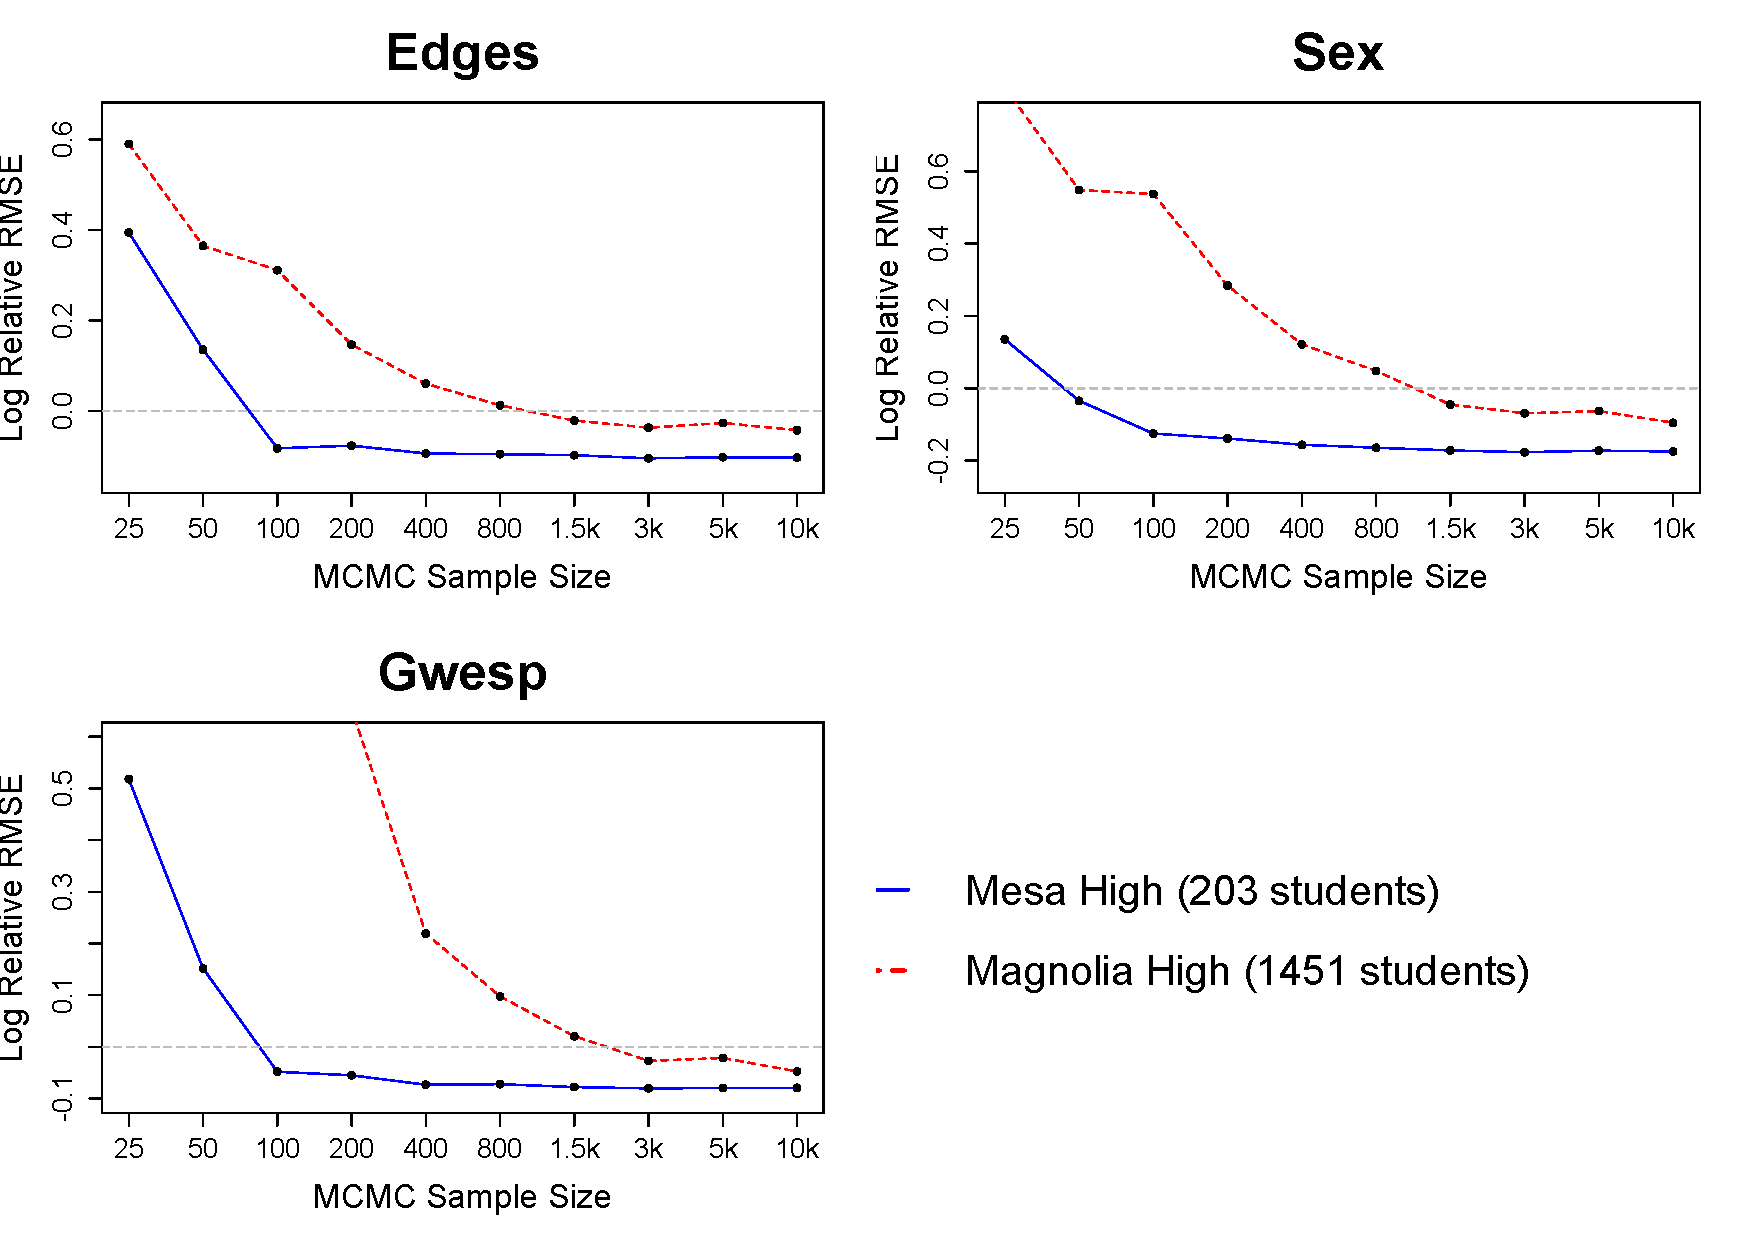
\includegraphics[scale=.34]{RMSE_presentation} 
\end{center}
\end{frame}

\begin{frame}
\frametitle{Parameter Estimation Method 2: Bootstrapped MPLE}
In contrast to the MPLE, the MCMLE does not underestimate the standard error.\\[0.4cm]
We introduce the \textbf{bootstrapped MPLE} in order to obtain more reliable confidence intervals:\\
\setbeamertemplate{enumerate items}[default]
\begin{enumerate}
\item Estimate the MPLE\\[0.2cm]
\item Simulate a reasonable number of networks (e.g. 500)\\[0.2cm]
\item Estimate the MPLE for each simulated network\\[0.2cm]
\item Take the 2.5th and 97.5th percentile to obtain a 95\% bootstrap confidence interval\\[0.2cm]
\end{enumerate}
\end{frame}




\begin{frame}
\frametitle{Bootstrapped MPLE vs. MCMLE: Coverage Probability}
\textbf{Treatment:} MCMLE as 'true' coefficients and simulate 1000 networks.\\[0.1cm] 
Calculate CI for each simulated network using bootstrapped MPLE, MCMLE and MPLE and report percentage the CI contains the 'true' value
\begin{center}
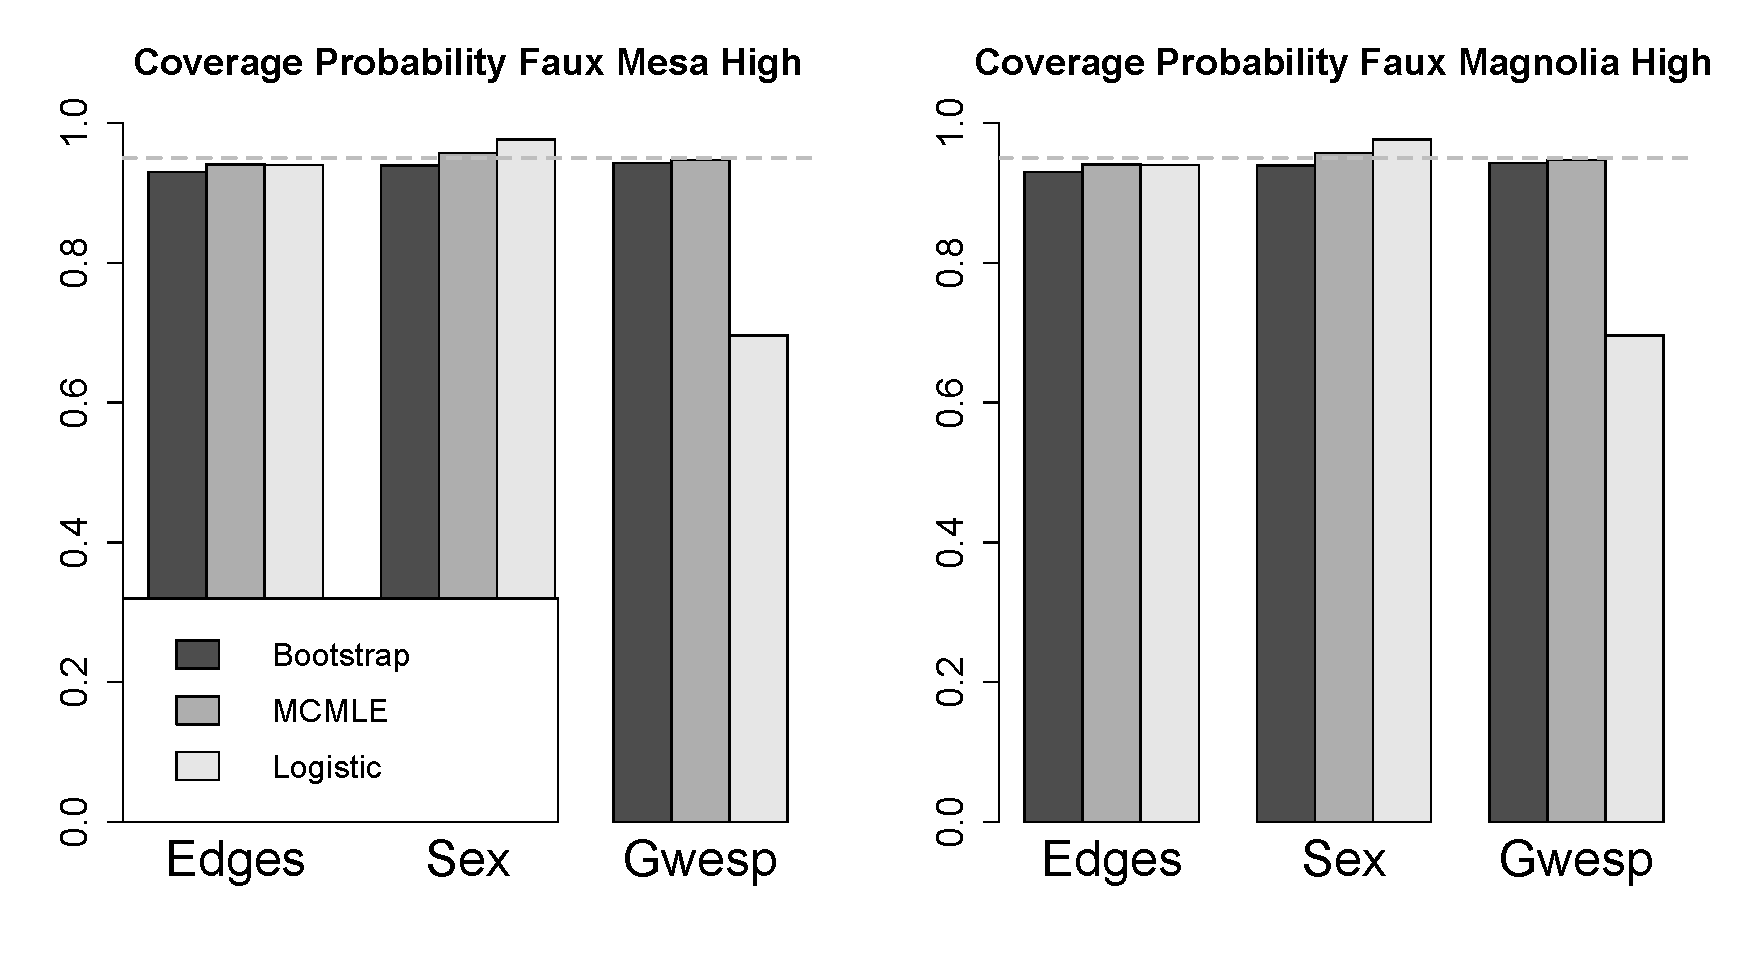
\includegraphics[scale=.4]{Coverage_presentation} 
\end{center}

\end{frame}

\begin{frame}
\frametitle{Bootstrapped MPLE vs. MCMLE: Computation Time}

$\bullet$ The bootstrapped MPLE is embarrassingly parallel.\\[0.2cm]
$\bullet$ By using multiple cores the computation time can be further reduced.\\[0.2cm]
This plot visualizes the time ratio of the bootstrapped MPLE to the MCMLE. 

\begin{center}
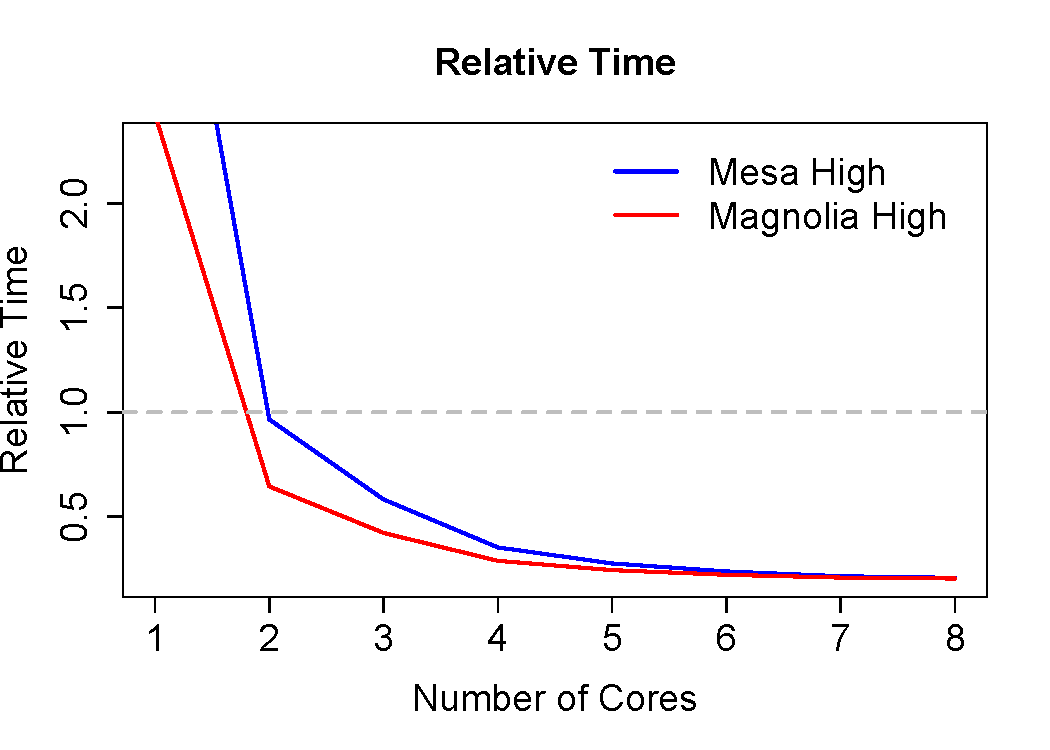
\includegraphics[scale=.46]{relative_time_presentation} 
\end{center}

\end{frame}

\begin{frame}
\frametitle{Assessing Degeneracy}
Degeneracy occurs if the stochastic process generated by the MCMC- algorithm does not hold through the model’s defined distribution as stationary distribution.
\begin{center}
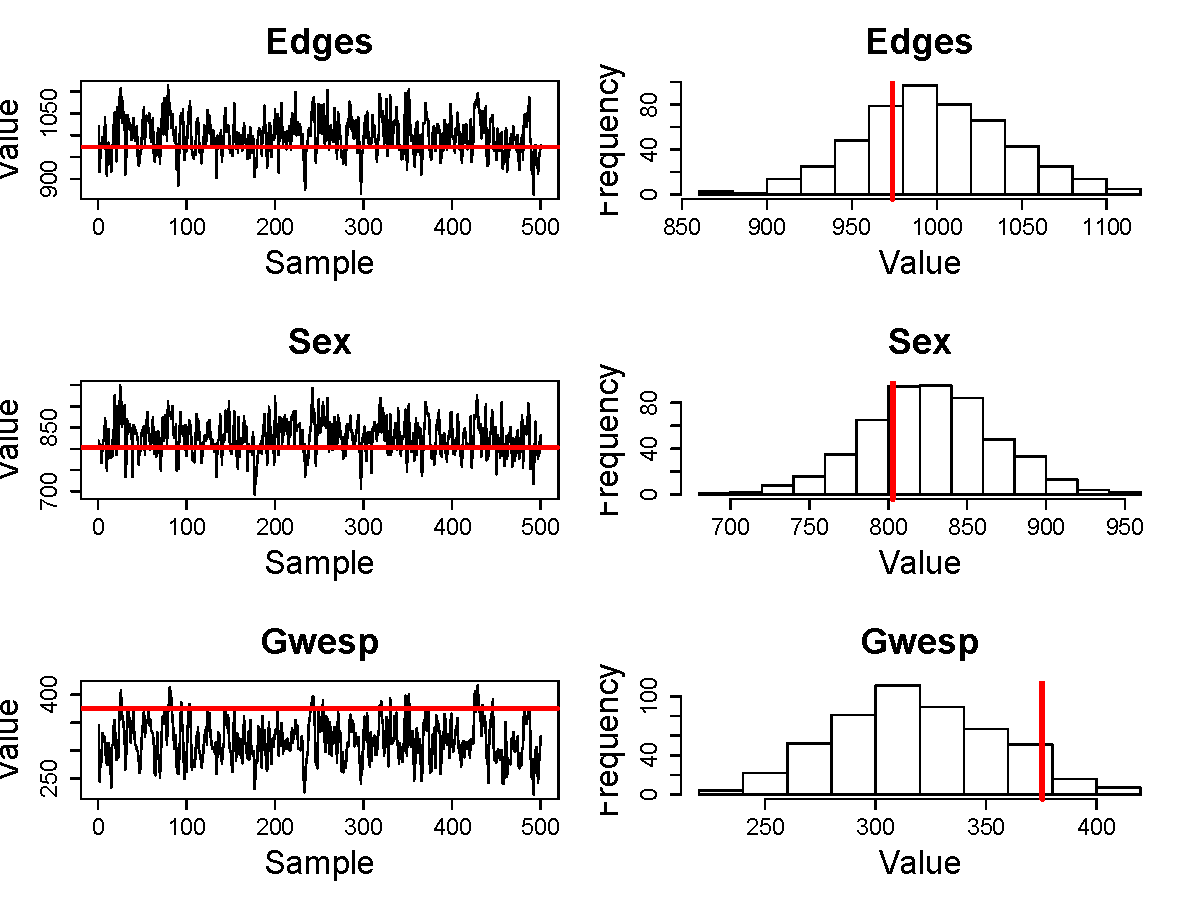
\includegraphics[scale=.4]{degeneracy_presentation} 
\end{center}
\end{frame}

\begin{frame}
\frametitle{Conclusion}
%MCMLE outperformed the two Bayesian methods in the simulation study. \\[0.2cm]
\begin{table}[]
\centering
\begin{tabular}{cll}
\hline
                      & \multicolumn{1}{c}{\textbf{Pros}}                                                                        & \multicolumn{1}{c}{\textbf{Cons}}                                                                         \\  \hline 
\multirow{2}{*}{\textbf{MCMLE}} & $\bullet$ approximately exact & $\bullet$ Computationally expensive            \\
                      &                                                                                                   $\bullet$ can assess degeneracy & \begin{tabular}[c]{@{}l@{}}$\bullet$ $\theta_0$ has to be picked  \\ close to $\theta$\medskip \end{tabular} \\ \hline
\multirow{2}{*}{\textbf{MPLE}} & $\bullet$ simple and fast & \multicolumn{1}{l}{$\bullet$ underestimates st. error}                                       \\ 
                      & \begin{tabular}[c]{@{}l@{}}$\bullet$ consistent estimator\medskip \end{tabular} &\\ \hline                                                                                               
\multirow{2}{*}{\textbf{b. MPLE}} & $\bullet$ simple and fast & \multicolumn{1}{l}{$\bullet$ slower than MPLE}                                       \\
                      & $\bullet$ can assess degeneracy & \\
                      & $\bullet$ consistent estimator& \\
                      & $\bullet$ reasonable CIs &
\end{tabular}
\end{table}
\end{frame}


\begin{frame}%[allowframebreaks]
  \frametitle{References}    
  \begin{thebibliography}{10}    
  \beamertemplatearticlebibitems
  \bibitem{Cranmer2011}
    B.A. Desmarais and S.J. Cranmer
    \newblock {\em Statistical mechanics of networks: Estimation and uncertainty}
    \newblock {\em Physica A}, 391(4):1865--1876, 2011.
    
  \beamertemplatearticlebibitems
  \bibitem{vanDuijn2009}
    M. van Duijn, K. Gile and M. Handcock
    \newblock {\em A framework for the comparison of maximum pseudo-likelihood and maximum likelihood estimation of exponential random graph models}
    \newblock {\em Social Networks}, 31(1):52--62, 2009.
    
\beamertemplatearticlebibitems
  \bibitem{Robins2007}
    G. Robins, P. Pattison, Y. Kalish and D. Lusher
    \newblock {\em An introduction to exponential random graph (p*) models for social networks}
    \newblock {\em Social Networks}, 29(2):173--191, 2007.    
    
    \beamertemplatearticlebibitems
  \bibitem{StraussIkeda}
    D. Strauss and M. Ikeda
    \newblock {\em Pseudolikelihood estimation for social networks}
    \newblock {\em JASA}, 85:204--212, 1990.
  \end{thebibliography}
\end{frame}

\begin{frame}
\frametitle{Simulating Networks with MCMC}
Choose a matrix $A^{(0)} \in \mathcal{A}(N)$ to start with and proceed as follows:\\
\begin{enumerate}
\item Randomly choose a dyad $A_{ij}:=A[i,j]$ where $i \neq j$ from $A^{(k)}$
\item Compute the value
$$\pi := \dfrac{\mathsf{P}(Y_{ij} \neq A_{ij}^{(k)} | Y_{ij}^c=A_{ij}^c, \theta_0)}{\mathsf{P}(Y_{ij}= A_{ij}^{(k)} | Y_{ij}^c=A_{ij}^c, \theta_0)}$$%= exp(\theta^T(\Gamma(A_{ij}^+)-\Gamma(A_{ij}^-)))$$
where $Y_{ij}^c=A_{ij}^c$ is short for $Y_{pq}=A_{pq}$ for all $(p,q)\neq (i,j)$.\\[0.2cm]
\item Fix $\delta:= \min\{1, \pi\}$ and draw a random number $Z$ from Bin$(1, \delta)$. If \\[0.2cm]
\begin{itemize}
\item $Z=0$, let $A^{(k+1)} := A^{(k)}$ \\[0.2cm]
\item $Z=1$, set $A_{ij}^{(k+1)}=1- A_{ij}^{(k)}$
\end{itemize}
\item Start at step 1 with $A^{(k+1)}$.
\end{enumerate}


\end{frame}


\end{document}